\section{Features HOWTO}
This section contains information about setting up various Dibbler
features. Since this section was added recently, it is not yet
comprehensive. That is expected to change.

\subsection{Leasequery}
\label{features-leasequery}
Servers provide addresses, prefixes and other configuration options to
the clients. Sometime administrators may want to obtain information
regarding certain leases, e.g. who has been given a specific address
or what addresses have been assigned to a specific client. This
mechanism is called Leasequery \cite{rfc5007}. New DHCPv6 participant
called requestor has been defined. Its sole purpose is to send queries
and receive responses. Dibbler provides example implementation. To
define a query, command line parameters are used. 

There are two types of queries: by address (who leases this address?)
and by client identifier (what addresses has this client?). To specify
one of such types, \verb+-addr+ or \verb+duid+ command-line switches
can be used. It is also mandatory to specify (using \verb+-i IFACE+),
which interface should be used to transmit the query.

Here is a complete list of all command-line switches:

\begin{description}
\item[-i IFACE] -- defines thru which interface should the query be sent
\item[-addr ADDR] -- sets query type to query by address. Also defines
  address, which the query will be about.
\item[-duid DUID] -- sets query type to query by client
  indentifier. Also defines client intentifier.
\item[-timeout SECS] -- specifies time, which requestor should wait
  for response.
\item[-dstaddr ADDR] -- destination address of the lease query
  message. By default messages are sent to the multicast address
  (ff02::1:2). To transmit query to an unicast addres, use this option.
\end{description}

Example query 1: Who has 2000::1 address?

\begin{lstlisting}
dibbler-requestor -i eth0 -addr 2000::1
\end{lstlisting}

Example query 2: Which addresses are assigned to client with specific client
identifier?

\begin{lstlisting}
dibbler-requestor -i eth0 -duid 00:01:00:01:0e:8d:a2:d7:00:08:54:04:a3:24
\end{lstlisting}

\subsection{Stateless vs stateful and IA, TA options}
\label{features-stateless-stateful}
This section explains the difference between stateless and stateful
configurations. IA and TA options usage is also described.

Usually, normal stateful configuration based on non-temporary
addresses should be used. If you don't know, what temporary addresses
are, you don't need them.

There are two kinds of configurations in DHCPv6 (\cite{rfc3315}, \cite{rfc3736}):
\begin{description}
  \item[stateful] -- it assumes that addresses (and possibly other parameters)
    are assigned to a client. To perform this kind of configuration,
    four messages are exchanged: \msg{SOLICIT}, \msg{ADVERTISE},
    \msg{REQUEST} and \msg{REPLY}.
  \item[stateless] -- when only parameters are configured (without
    assigning addresses to a client). During execution of this type of
    configuration, only two messages are exchanged: \msg{INF-REQUEST}
    and \msg{REPLY}.
\end{description}

During normal operation, client works in a stateful mode. If not
instructed otherwise, it will request one or more normal (i.e. non-temporary)
address. It will use \opt{IA} option (Identity Association for
Non-temporary Addresses, see \cite{rfc3315} for details) to request
and retrieve addresses. Since this is a default behavior, it does not
have to be mentioned in the client configuration
file. Nevertheless, it can be provided:

\begin{lstlisting}
# client.conf
iface eth0 {
  ia
  option dns-server
}
\end{lstlisting}

In a specific circustances, client might be interested in obtaining
only temporary addresses. Although this is still a stateful mode, its
configuration is sligtly different. There is a special option called \opt{TA}
(Identity Association for Temporary Addresses, see \cite{rfc3315} for
details). This option will be used to request and receive temporary
addresses from the client. To force client to request temporary
addresses instead of permanent ones, \verb+ta+ keyword must be used in
client.conf file. If this option is defined, only temporary address
will be requested. Keep in mind that temporary addresses are not
renewed.

\begin{lstlisting}
# client.conf
iface eth0 {
  ta
  option dns-server
}
\end{lstlisting}

It is also possible to instruct client to work in a stateless mode. It
will not ask for any type of addresses, but will ask for specific
non-adress related configuration parameters, e.g. DNS Servers
information. This can be achieved by using \verb+stateless+
keyword. Since this is a global parameter, it is not defined on any
interface, but as a global option.

\begin{lstlisting}
# client.conf
stateless
iface eth0
{
  option dns-server
}
\end{lstlisting}

Some of the cases mentioned above can be used together. However,
several combinations are illegal. Here is a complete list:
\begin{description}
\item[none] -- When no option is specified, client will assume one IA
	   with one address should be requested. Client will send
	   \verb+ia+ option (stateful autoconfiguration).
\item[ia] -- Client will send \verb+ia+ option (stateful
  autoconfiguration).
\item[ia,ta] -- When both options are specified, client will request
  for both - Non-temporary as well as Temporary addresses (stateful
  autoconfiguration).
\item[stateless] -- Client will request additional configration
  parameters only and will not ask for addresses (stateless
  autoconfiguration).
\item[stateless,ia] -- This combination is not allowed.
\item[stateless,ta] -- This combination is not allowed.
\item[stateless,ia,ta] -- This combination is not allowed.
\end{description}

\subsection{DNS Update}
\label{features-fqdn}
\Note In this section, we will assume that hostnames will be used
from the example.com domain and that addresses will be provided from the
2000::/64 pool. 

\begin{figure}[ht]
\begin{center}
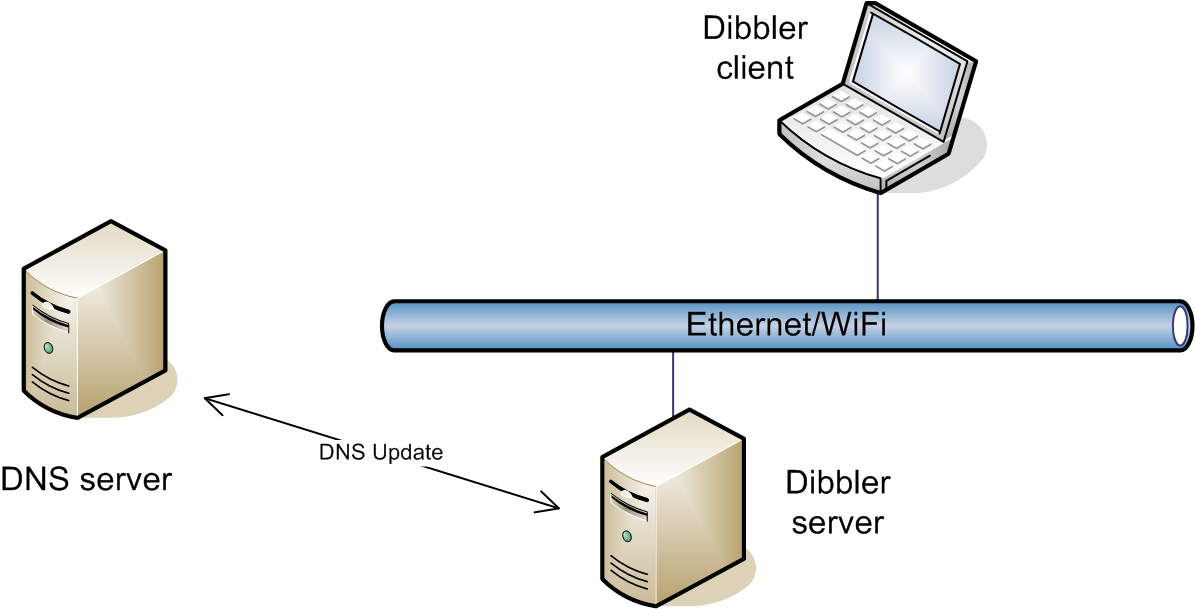
\includegraphics[width=0.65\textwidth]{dibbler-fqdn-srv-update}
\caption{\emph{DNS Update (performed by server)}}
\end{center}
\end{figure}

During normal operation, DHCPv6 client receives one or more IPv6 address(es)
from DHCPv6 server. If configured to do so, it can also receive
information about DNS server addresses. As an additional service, DNS
Update can be performed. This feature, sometimes known as Dynamic DNS,
keeps DNS entries up to date. When client boots, it gets its fully
qualified domain name and this name can be used to reach this
particular client by other nodes. Details of this mechanism is described
in \cite{rfc4704}.

There are two types of the DNS Updates. First is a so called forward
resolving. It allows to change a node's name into its address,
e.g. malcolm.example.com can be translated into 2000::123. Other kind
of record, which can be updated is a so called reverse resolving. It
allows to obtain full name of a node with know address, e.g. 2000::124
can be translated into zoe.example.com.

To configure this feature, following steps must be performed:

\begin{enumerate}
\item Configure DNS server. DNS server supporting IPv6 and dynamic
  updates must be configured. One example of such server is a BIND
  9.3. It is necessary to allow listening on the IPv6 sockets and
  define that specific domain can be updated. See example below.
\item Configure Dibbler server to provide DNS server informations for
  clients. DNS Updates will be sent to the first DNS server on the
  list of available servers.
\item Configure Dibbler server to work in stateful mode, i.e. that it
  can provide addresses for the clients. This is a default mode, so
  unless configuration was altered, this step is already done. Make
  sure that there is no ,,stateless'' keyword in the
  \verb+server.conf+ file.
\item Define list of the available names in the server configuration
  file. Make sure to use fully qualified domain names
  (e.g. malcolm.example.com), not the hostnames only. 
\item Configure dibbler client to request for DNS Update. Use ,,option
  fqdn'' to achieve this. 
\item Server can be configured to execute 
      \begin{itemize}
       \item both (AAAA and PTR) updates by itself
       \item execute PTR only by itself and let client execute AAAA
	     update
       \item don't perform any updates and let client perform AAAA
	     update.
      \end{itemize}
\end{enumerate}

Note that only server is allowed to execute PTR updates. After
configuration, client and/or server should log following line, which
informs that Dynamic DNS Update was completed successfully.

\begin{verbatim}
2006.07.24 01:52:51 Client Notice    FQDN Configured successfully !
\end{verbatim}

\begin{figure}[ht]
\begin{center}
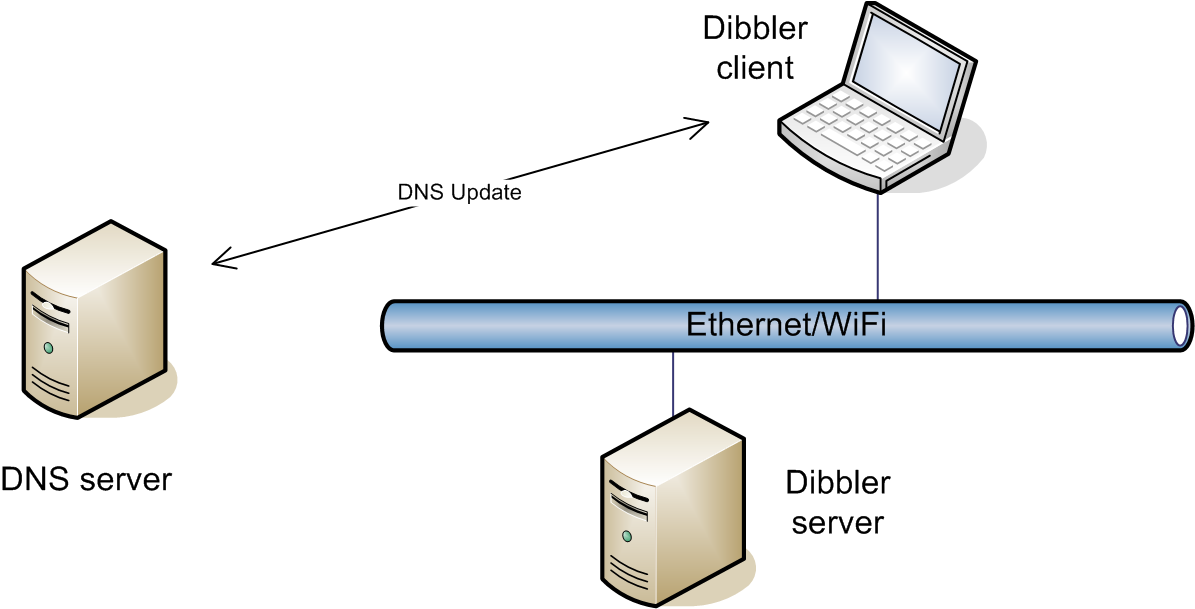
\includegraphics[width=0.65\textwidth]{dibbler-fqdn-cli-update}
\caption{\emph{DNS Update (performed by client)}}
\end{center}
\end{figure}

\subsubsection{Example BIND configuration}
Below are example configuration files for the BIND 9.3. First is a
relevant part of the /etc/bind/named.conf configuration file. Generally,
support for IPv6 in BIND is enabled (listen-on-v6) and there are two
zones added: example.com (normal domain) and
0.0.0.0.0.0.0.0.0.0.0.0.0.0.0.2.ip6.arpa (reverse
mapping). Corresponding files are stored in \verb+example.com+ and
\verb+rev-2000+ files. For details about meaning of those directives,
please consult \emph{BIND 9 Administrator Reference Manual}.

\Note Provided configuration is not safe from the security point of
view. See next subsection for details.
  
\begin{lstlisting}
// part of the /etc/bind/named.conf configuration file
options {
    listen-on-v6 { any; };
    listen-on    { any; };

    // other global options here
    // ...
};

zone "example.com" {
    type master;
    file "example.com";
    allow-update   { any; };
    allow-transfer { any; };
    allow-query    { any; };

    // other example.com domain-specific 
    // options follow
    // ...
};

zone "0.0.0.0.0.0.0.0.0.0.0.0.0.0.0.2.ip6.arpa" {
    type master;
    file "rev-2000";
    allow-update   { any; };
    allow-transfer { any; };
    allow-query    { any; };

   // other 2000::/64 reverse domain related 
   // options follow
   // ...
};
\end{lstlisting}

% \vspace{-0.3cm}
% \begin{center}
% BIND's named.conf example
% \end{center}

Below are examples of two files: forward and reverse zone. First example
presents how to configure normal domain. As an example there is entry
provided for zoe.example.com host, which has 2000::123 address. Note
that you do not have to manually configure such entries -- dibbler will
do this automatically. It was merely provided as an example, what kind
of mapping will be done in this zone.

\begin{lstlisting}
; 
$ORIGIN .
$TTL 86400      ; 1 day
example.com             IN SOA  v13.klub.com.pl. root.v13.klub.com.pl. (
                                129        ; serial
                                7200       ; refresh (2 hours)
                                3600       ; retry (1 hour)
                                604800     ; expire (1 week)
                                86400      ; minimum (1 day)
                                )
                        NS      v13.klub.com.pl.
                        A       1.2.3.4
                        TXT     "Fake domain used for Dibbler tests."
$ORIGIN example.com.
$TTL 7200       ; 2 hours
zoe                     AAAA    2000::123
\end{lstlisting}

Second example presents zone file for reverse mapping. It contains
entries for a special zone called
0.0.0.0.0.0.0.0.0.0.0.0.0.0.0.2.ip6.arpa. This zone represents 2000::/64
address space. As an example there is a static entry, which maps address
2000::999 to a canonical name kaylee.example.com. Note that you do not
have to manually configure such entries -- dibbler will do this
automatically. It was merely provided as an example, what kind
of mapping will be done in this zone.

\begin{lstlisting}
; rev-2000 example file
$ORIGIN .
$TTL 259200     ; 3 days

; this line below is split in two due to page with limitation
0.0.0.0.0.0.0.0.0.0.0.0.0.0.0.2.ip6.arpa IN 
      SOA 0.0.0.0.0.0.0.0.0.0.0.0.0.0.0.2.ip6.arpa. hostmaster.ep.net. (
; this line above is split in two due to page with limitation
                                200608268  ; serial
                                86400      ; refresh (1 day)
                                1800       ; retry (30 minutes)
                                172800     ; expire (2 days)
                                259200     ; minimum (3 days)
                                )
                        NS      klub.com.pl.
$ORIGIN 0.0.0.0.0.0.0.0.0.0.0.0.0.0.0.0.0.0.0.0.0.0.0.0.0.0.0.0.2.ip6.arpa.
$TTL 86200      ; 23 hours 56 minutes 40 seconds
3.2.1                   PTR     picard.example.com.

; this line below is split in two due to page with limitation
9.9.9                   PTR     kaylee.example.com.
$ORIGIN 0.0.0.0.0.0.0.0.0.0.0.0.0.0.0.2.ip6.arpa.

; example entry: 2000::999 -> troi.example.com.
; this line below is split in two due to page with limitation
9.9.9.0.0.0.0.0.0.0.0.0.0.0.0.0.0.0.0.0.0.0.0.0.0.0.0.0.0.0.0.2.ip6.arpa 
      PTR troi.example.com.
; this line above is split in two due to page with limitation
\end{lstlisting}
\Note Due to page width limitation, if the example above, two lines were
split. 
%% $

\subsubsection{Dynamic DNS Testing and tips}
Proper configuration of the DNS Update mechanism is not an easy
task. Therefore this section provides description of several methods of
testing and tuning BIND configuration. Please review following steps
before reporting issues to the author or on the mailing list.

\begin{itemize}
\item See example server and client configuration files described in a
      sections \ref{example-client-fqdn} and \ref{example-server-fqdn}. Also
      note that Dibbler distribution should be accompanied with several
      example configuration files. Some of them include FQDN usage examples.
\item Make sure that unix user, which runs BIND, is able to create and
      write file example.com.jnl. When BIND is unable to create this
      journal file, it will fail to accept updates from dibbler and will
      report failure. Check BIND log files, which are usually stored in the
      \verb+/var/log/+ directory.
\item Make sure that you have routing configured properly on a host,
      which will attempt to perform DNS Update. Use ping6 command to
      verify that DNS server is reachable from this host.
\item Make sure that your DNS server is configured properly. To do so,
      you might want to use \verb+nsupdate+ tool. It is part of the BIND
      distribution, but it is sometimes distributed separated as part of
      the dnsutils package. After executing nsupdate tool, specify
      address of the DNS server (\verb+server+ command), specify update
      parameters (\verb+update+ command) and then type \verb+send+. If
      nsupdate return a command prompt, then the update was
      successful. Otherwise nsupdate will print DNS server's response,
      e.g. NOTAUTH of SRVFAIL. See below for examples of successful
      forward (AAAA record) and reverse (PTR record) updates.
\item After DNS Update is performed, DNS records can be verified using
      dig command line tool (a part of the dnsutils package). Command
      syntax is: 
      \verb+dig @(dns-server-address) name record-type+. 
      In the following example, this query checks for name
      jayne.example.com at a server located at 2000::1 address. Record
      type AAAA (standard record for resolving name into IPv6 address)
      is requested. dig tool provides server's response in the
      \verb+ANSWER SECTION:+. See example log below.
\item In example BIND configuration above, zone transfers, queries and
      updates are allowed from anywhere. To make this configuration more
      secure, it might be a good idea to allow updates only from a
      certain range of addresses or even one (DHCPv6 server's) address
      only.
\end{itemize}


%%%%%%%%%%%%%%%%%%%%%%%%%%%%%%%%%%%%%%%%%%%%%%%%%%%%%%%%%%%%%%%%%%%%%%%%%%%%%%%%

To manually make AAAA record update, type:
\begin{lstlisting}
nsupdate
>server 2000::1
>update add worf.example.com 7200 IN AAAA 2000::567
>send
\end{lstlisting}

To manually make PTR record update, type:
\begin{lstlisting}
nsupdate
>server 2000::1
>update add 
3.2.1.0.0.0.0.0.0.0.0.0.0.0.0.0.0.0.0.0.0.0.0.0.0.0.0.0.0.0.0.2.ip6.arpa.
86200 IN PTR picard.example.com. 
>send
\end{lstlisting}

\Note Everything between "update" and "picard.example.com" must be typed in one line.

And here is an example dig session:

\begin{lstlisting}
v13:/var# dig @2000::1 jayne.example.com AAAA
; <<>> DiG 9.3.2 <<>> @2000::1 jayne.example.com AAAA
; (1 server found)
;; global options:  printcmd
;; Got answer:
;; ->>HEADER<<- opcode: QUERY, status: NOERROR, id: 33416
;; flags: qr aa rd ra; QUERY: 1, ANSWER: 1, AUTHORITY: 1, ADDITIONAL: 2

;; QUESTION SECTION:
;jayne.example.com.             IN      AAAA

;; ANSWER SECTION:
jayne.example.com.      7200    IN      AAAA    2001::e4

;; AUTHORITY SECTION:
example.com.            86400   IN      NS      v13.klub.com.pl.

;; Query time: 6 msec
;; SERVER: 2000::1#53(2000::1)
;; WHEN: Mon Jul 24 01:38:13 2006
;; MSG SIZE  rcvd: 136
\end{lstlisting}
%% >>

\subsubsection{Accepting Unknown FQDNs}
By default, server configured to support FQDN has a list of names that
are to be provided to clients. But there are scenarios, where client
uses it own name and sends it to the server. So it makes sense to
sometimes allow client's own domain names. Server does not know
anything about such names, thus its nickname ''Unknown FQDN''.

To configure such support, add \verb+accept-unknonwn-fqdn+ option to
the interface. For example:

\begin{lstlisting}
iface "eth0" {

# assign addresses from this class
 class {
   pool 2000::/64
 }

# provide DNS server location to the clients
# also server will use this address to perform DNS Update,
# so it must be valid and DNS server must accept DNS Updates.
 option dns-server 2000::1
 
# provide their domain name
 option domain example.com

# provide fully qualified domain names for clients
# note that first, second and third entry is reserved
# for a specific address or a DUID

 option fqdn 1 64
             zebuline.example.com - 2000::1,
	     kael.example.com - 2000::2,
	     wash.example.com - 0x0001000043ce25b40013d4024bf5,
	     zoe.example.com,
	     malcolm.example.com,
	     kaylee.example.com,
	     jayne.example.com,
	     inara.example.com

 accept-unknown-fqdn
	     
}
\end{lstlisting}

\subsection{Server address caching}
Previous Dibbler versions assigned a random address from the available
address pool, so the same client received different address each time it
asked for one. In the 0.5.0 release, new mechanism was introduced
to make sure that the same client gets the same address each time. It is
called \emph{Server caching}.

Below is the algorithm used by the server to assign an address to the client.

\begin{itemize}
 \item if the client provided hint, it is valid (i.e. is part of the
       supported address pool) and not used, then assign requested address.
 \item if the client provided hint, it is valid (i.e. is part of the 
       supported address pool) but used, then assign free address from
       the same pool.
 \item if the client provided hint, but it is not valid (i.e. is not
       part of the supported address pool, is link-local or a multicast
       address), then ignore the hint completety.
 \item if the did not provide valid hint (or provided invalid one), try
       to assign address previously assigned to this client (address caching)
 \item if this is the first time the client is seen, assign any address
       available.
\end{itemize}
%% see SrvOptions/SrvOptIA_NA.cpp, TSrvOptIA_NA::getFreeAddr() method

\subsection{Relays}
\label{features-relays}
In small networks, all nodes (server, hosts and routers) are connected
to the same network segment -- usually Ethernet segment or a single
access point or hotspot. This is very convenient as all clients can
reach server directly. However, larger networks usually are connected
via routers, so direct communication is not always possible. On the
other hand it is useful to have one server, which supports multiple
links -- some connected directly and some remotely.

\begin{figure}[ht]
\begin{center}
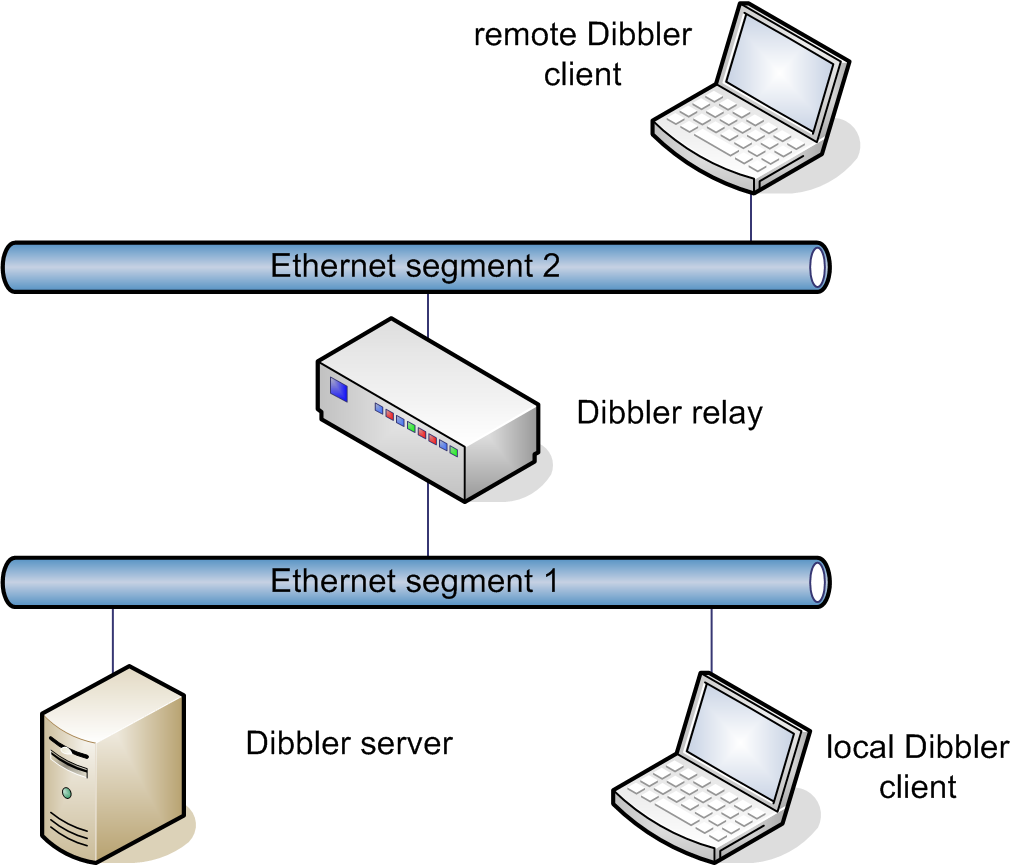
\includegraphics[width=0.65\textwidth]{dibbler-relay}
\caption{\emph{Relay deployment}}
\end{center}
\end{figure}

Very nice feature of the relays is that they appear as actual servers
from the client's point of view. Therefore no special arrangement or
configuration on the client side is required. On the other hand, from
the administrator point of view, it is much easier to manage one DHCPv6
server and deploy several relays than manage several servers on remote
links. 

It is important to understand that relays not simply forward DHCPv6
messages. Each message forwarded from client to the server is
encapsulated. Also each message forwarded from server to a client is
decapsulated. Therefore additional server configuration is required to
deal with encapsulated (i.e. relayed) traffic.

To avoid confusion during reference to a specific link (i.e. eth0 on
the relay may be different link than eth0 on the server), each link
must be referred to using its unique interface-id. For simplicity
reasons, Dibbler uses 4 bytes long identifiers, which are specified as
numbers. It is essential to use the same indentifier in the relay
configuration as well as in the server, so both will refer to the same
link using the same number. See section \ref{example-server-relay1} for
example how to configure server and section \ref{example-relay-1} for 
corresponding relay configuration.

\begin{figure}[ht]
\begin{center}
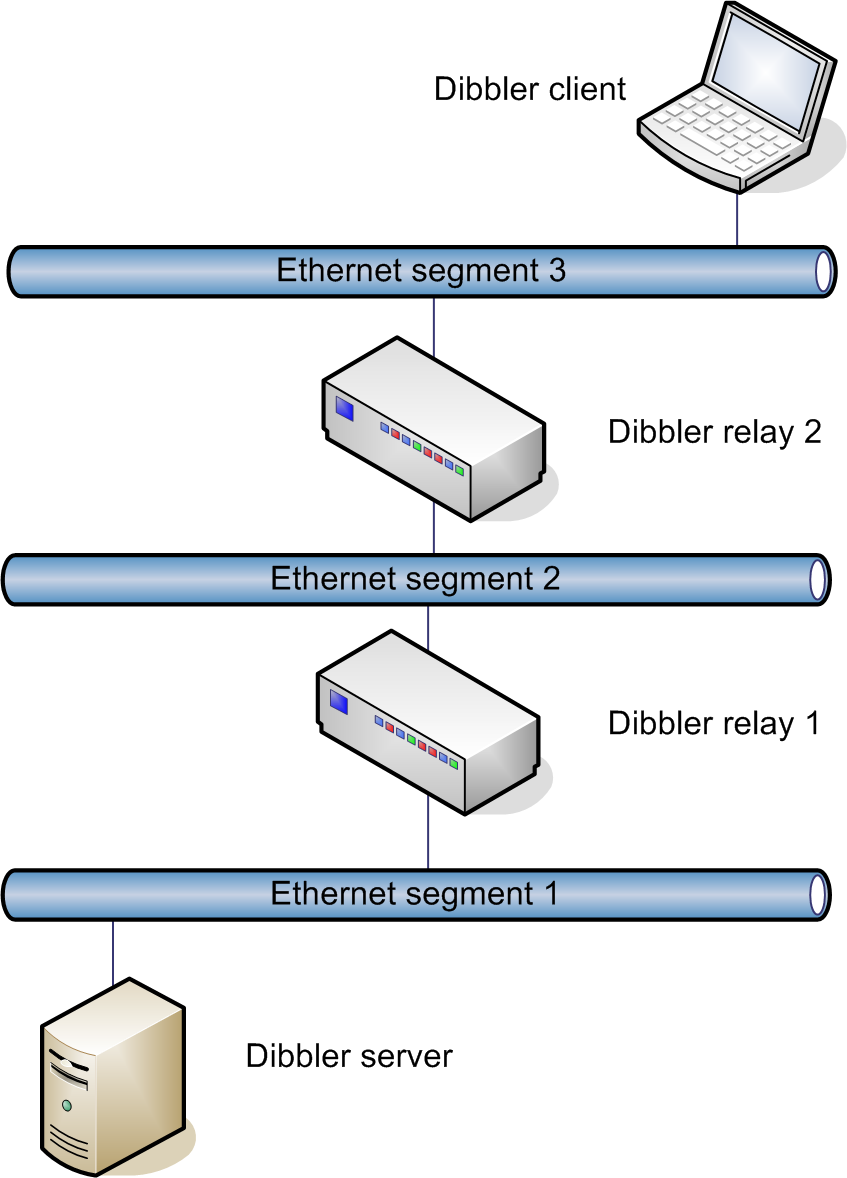
\includegraphics[width=0.4\textwidth]{dibbler-cascade-relays}
\caption{\emph{Cascade relays}}
\label{fig-cascade-relays}
\end{center}
\end{figure}

In larger networks it is sometimes useful to connect multiple
relays. Assuming there are 2 relays connecting server and client. Such
scenario is depicted on figure \ref{fig-cascade-relays}. Requests from
client are received by relay2, which encapsulates and sends them to
relay1. Relay1 further encapsulates those messages and sends them to
the server. Since server receives double encapsulated messages, it
must be properly configured to support such traffic. See section
\ref{example-server-relay2} for details about server configuration and 
section \ref{example-relay-cascade} for example relays configuration.

\subsection{XML files}
\label{features-xml}
During its execution, all dibbler components (client, server and
relay) store its internal information in the XML files. In Linux
systems, they are stored in the \verb+/var/lib/dibbler+ directory. In
Windows, current directory (i.e. directory where exe files are
located) is used instead. There are several xml files generated. Since
they are similar for each component, following list provides
description for server only:

\begin{itemize}
\item server-CfgMgr.xml -- Represents information read from a
  configuration file, e.g. available address pool or DNS server
      configuration.
\item server-IfaceMgr.xml -- Represens detected interfaces in the
  operating system, as well as bound sockets and similar information.
\item server-AddrMgr.xml -- This is database, which contains identity
  associations with associated addresses.
 \item server-cache.xml -- Since caching is implemented by the server
      only, this file is only created by the server. It contains
      information about previously assigned addresses. 
\end{itemize}

\subsection{Prefix delegation}
\label{features-prefix}
According to \cite{rfc3633}: 

\begin{quote}
   The prefix delegation mechanism is
   intended for simple delegation of prefixes from a delegating router
   to requesting routers.  It is appropriate for situations in which the
   delegating router does not have knowledge about the topology of the
   networks to which the requesting router is attached, and the
   delegating router does not require other information aside from the
   identity of the requesting router to choose a prefix for delegation.
   For example, these options would be used by a service provider to
   assign a prefix to a Customer Premise Equipment (CPE) device acting
   as a router between the subscriber's internal network and the service
   provider's core network.
\end{quote}

\begin{figure}[ht]
\begin{center}
\label{fig-prefixes-host}
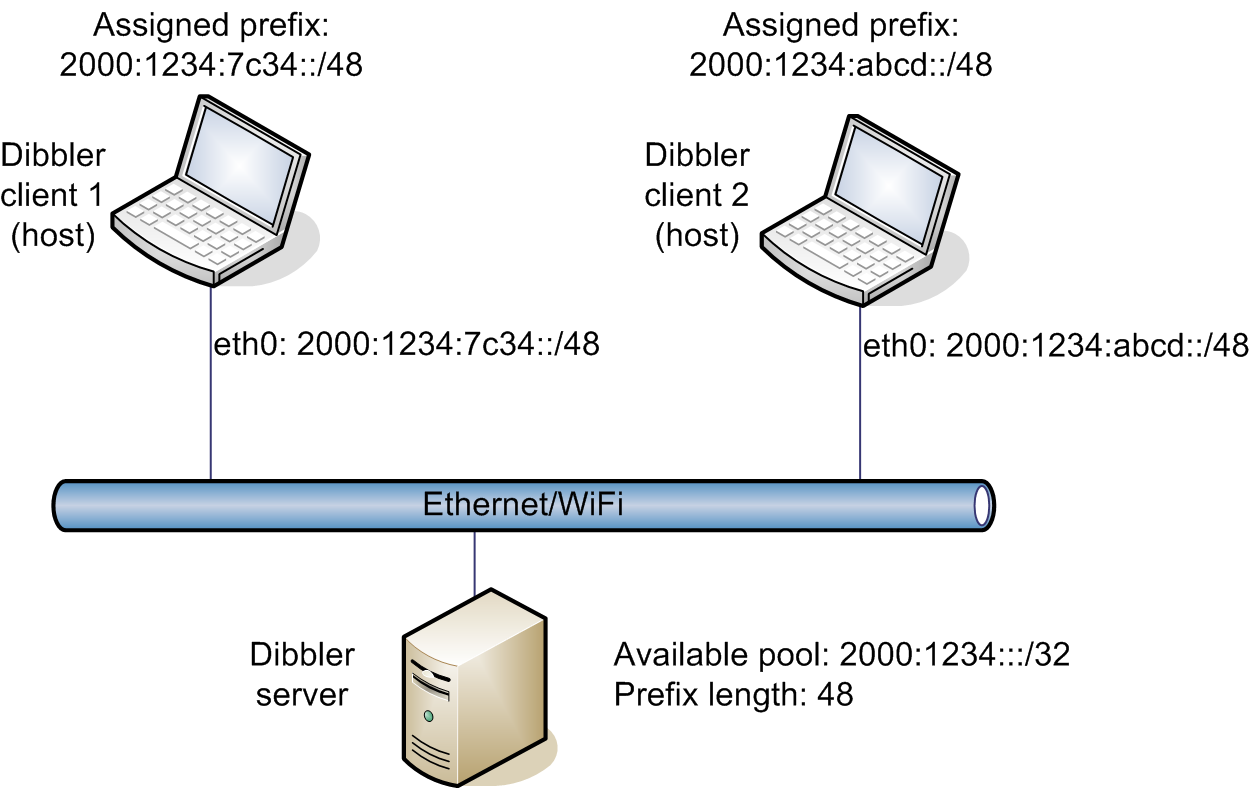
\includegraphics[width=0.65\textwidth]{dibbler-prefixes-host}
\caption{\emph{Prefix delegation (host behaviour)}}
\end{center}
\end{figure}

To configure server to provide prefixes, a pool must be defined and
also client prefixes' length. For example section below assigns
2000:1234::/32 pool to be managed by this server. From this pool,
server will assign /48 prefixes to the clients. For example, client
can receive prefix 2000:1234:7c34::/48. 

\begin{lstlisting}
pd-class {
    pd-pool 2000:1234::/32
    pd-length 48
}
\end{lstlisting}

As a general rule, server will provide random prefix to a client,
unless client provided a hint. The full prefix assignment algorithm is
as follows:

\begin{enumerate}
\item client didn't provide any hints: one prefix from each pool will
  be granted
\item client has provided hint and that is valid (supported and
  unused): requested prefix will be granted
\item client has provided hint, which belongs to supported pool, but this prefix is used:
  other prefix from that pool will be asigned
\item client has provided hint, but it is invalid (not beloninging to
  a supported pool, multicast or link-local): see point 1
\end{enumerate}

Dibbler implementation supports prefix delegation, but it also
extends it. From the server point of view, everything works according
to specs \cite{rfc3633}. However, client is able to meaningfully use
received prefix, even when packet forwarding is not enabled
(i.e. client is a host, not a router). In fact, this is simpler
scenario, therefore it will be explained first. This scenario is
depicted on Fig. \ref{fig-prefixes-host}. When dibbler client receives
prefix and detects that packet forwarding in not enabled, it will
configure received prefix on the interface, which data has been
received on.

Client's behavior is radically different if packet forwarding is
enabled (i.e. client is a router, not a host). In such scenario, when
client receives prefix on one interface (e.g. prefix
2000:1234:7c34::/48 received on eth0) it will generate subprefixes for
all other interfaces, which are up, running, non-loopback and
multicast capable. In the example depicted on
Fig. \ref{fig-prefixes-router}, received prefix was split into 3
prefixes: 2000:1234:7c34:1000::/56 for eth1, 2000:1234:7c34:2000::/56 for eth2
and 2000:1234:7c34:3000::/56 for eth3.

\begin{figure}[ht]
\begin{center}
\label{fig-prefixes-router}
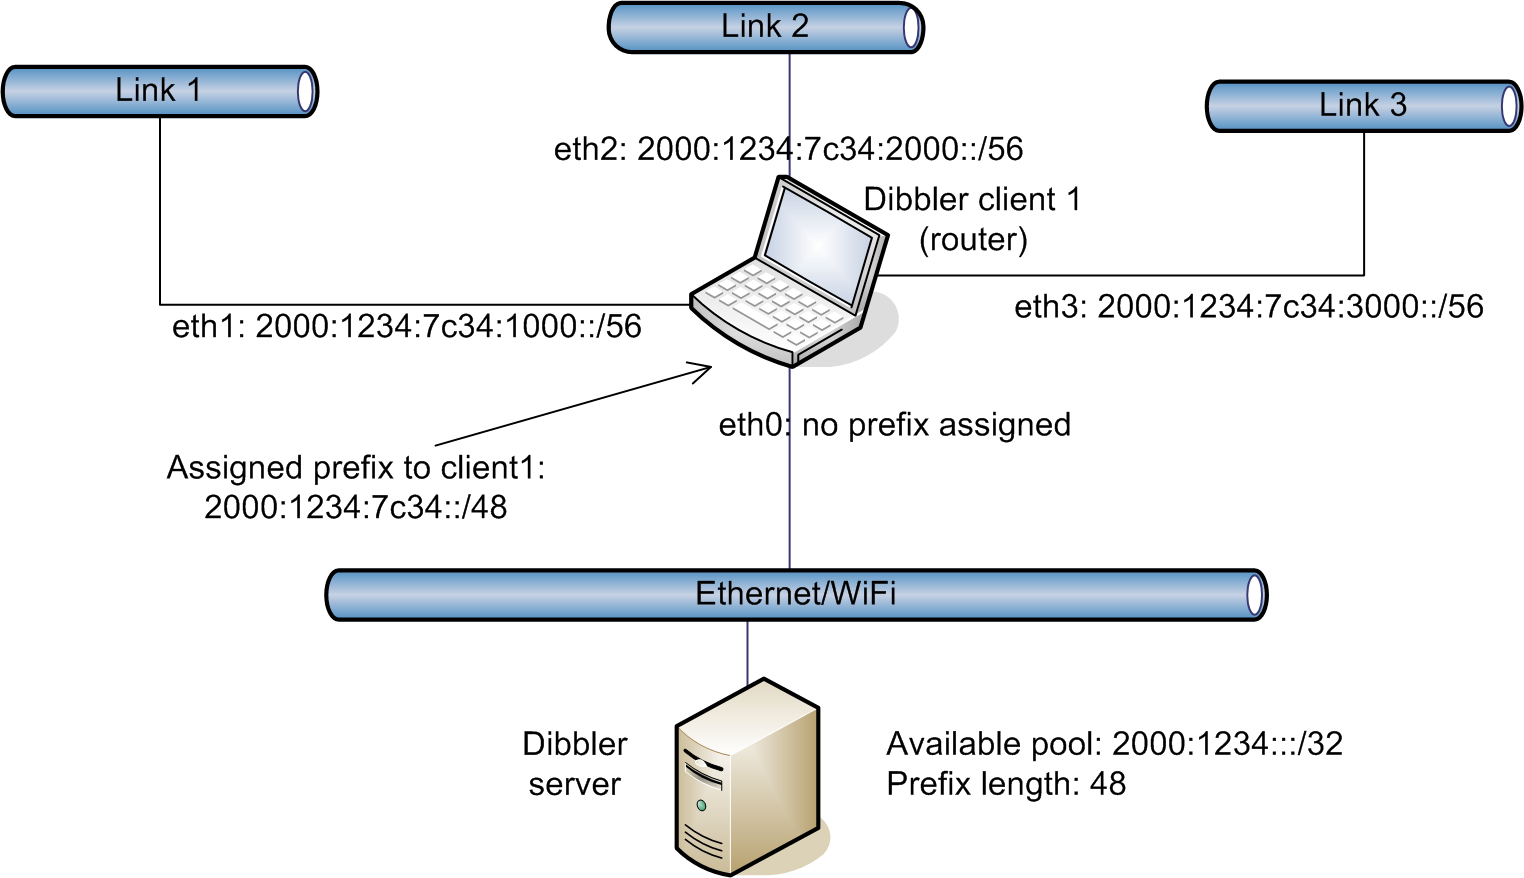
\includegraphics[width=0.65\textwidth]{dibbler-prefixes-router}
\caption{\emph{Prefix delegation (router behaviour)}}
\end{center}
\end{figure}

It is also possible to define multiple prefix pools. See section
\ref{example-server-prefix} for simple prefix delegation configuration
for server or section \ref{example-server-prefixes} for multiple
prefixes configuration. Also section \ref{example-client-prefix}
provides information related to client configuration.

\subsection{Authentication and Authorization}
\label{features-auth}

Implementation of authentication and authorization in Dibbler is
loosely based on \cite{draft-aaa}. Mainly option formats have been
used, for interoperability purposes. Draft does not specify how to
communicate with home and foreign AAA servers (AAAH and AAAF) using
Diameter or Radius protocol, so Dibbler uses a different, simpler
approach. Keys are stored locally in files. (see Fig. \ref{fig-aaa}).

\begin{figure}[ht]
\begin{center}
\label{fig-aaa}
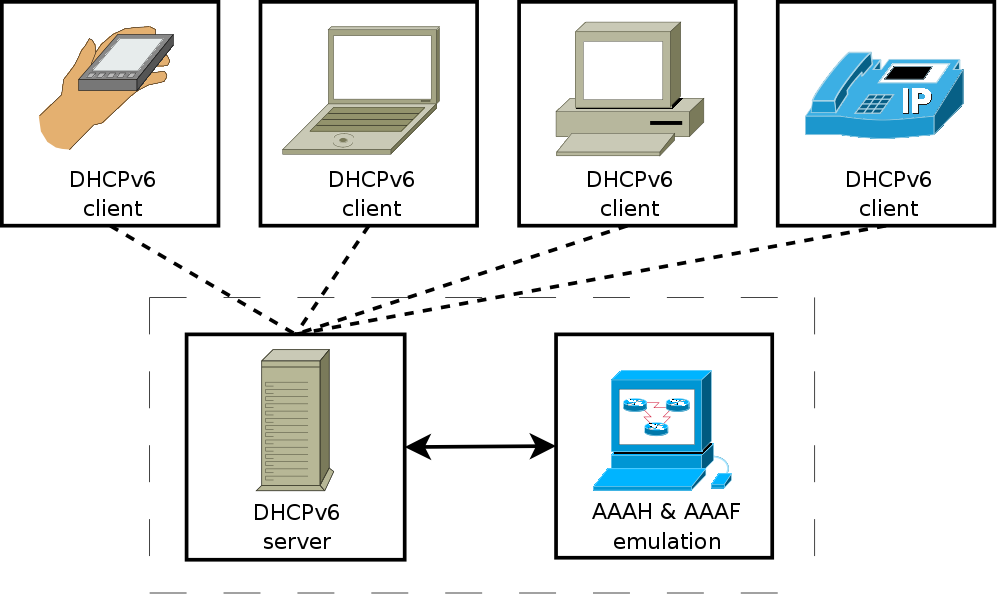
\includegraphics[width=0.65\textwidth]{dibbler-aaa}
\caption{\emph{Simplified model of AAA}}
\end{center}
\end{figure}

For each pair of client and server three files are needed. Client uses
a file \texttt{AAA-SPI}, which contains 32-bit AAA-SPI (AAA Security
Parameter Index) --- eight hexadecimal digits, to properly introduce
himself (authorize) to server. Also it needs file named \texttt{AAA-key-\textit{AAASPI}},
which contains a key that is used to generate authentication information
in AAAAUTH and AUTH options. The AAA-key is any number of arbitrary chosen
bytes and is generated by administrator of DHCPv6 server. The server needs
only one file per client to properly communicate using authentication. The
file is named \texttt{AAA-key-\textit{AAASPI}}, where \textit{AAASPI} is the
same value, that client has in \texttt{AAA-SPI} file. This file contains the
same AAA-key, that client has in \texttt{AAA-key} file. Dibbler searches for
those files in \textit{AAA directory}, which is \texttt{/var/lib/dibbler/AAA}
when running under Linux and current directory, when running under Windows.

Typical scenario of preparing a client and server to use authentication:
\begin{enumerate}
 \item Administrator generates \texttt{AAA-key-\textit{AAASPI}} file. \textit{AAASPI}
is an arbitrary chosen 32-bit number (as described above). The file contains any AAA-key
and can be administrator's favorite poem or can be simply generated using \texttt{dd}
and \texttt{/dev/urandom}:
\begin{lstlisting}
$ dd if=/dev/urandom of=AAA-key-b9a6452c bs=1 count=32
\end{lstlisting}
%%$

\item Administrator creates file \texttt{AAA-SPI} which contains previously chosen
\textit{AAASPI}. This file will be used by the client only.

\item Administrator transfers \texttt{AAA-SPI} and \texttt{AAA-key-\textit{AAASPI}} to the client, using
some secure method (e.g. mail+PGP, scp, https) to avoid sniffing the key by a potential
attacker.

\item Client: User stores \texttt{AAA-SPI} and \texttt{AAA-key-\textit{AAASPI}} in \textit{AAA directory}.

\item Server: Administrator stores \texttt{AAA-key-\textit{AAASPI}} in \textit{AAA directory}.

\end{enumerate}

For example, configuration files can look like this:

\begin{itemize}
\item Server's \texttt{AAA-key-b9a6452c} and client's \texttt{AAA-key} (32 bytes):
\begin{lstlisting}
ma8s9849pujhaw09y4h[80pashydp80f
\end{lstlisting}

\item Client's \texttt{AAA-SPI} (8 bytes):
\begin{lstlisting}
b9a6452c
\end{lstlisting}
\end{itemize}

When configuration files are prepared and stored in client's and server's
\textit{AAA directory} you are ready to use authentication. For detailed description
of possible options see \ref{client-conf-extension}. For quick start:
\begin{itemize}
 \item set ``\texttt{auth-enabled true}'' in \texttt{client.conf}

 \item set ``\texttt{auth-method digest-hmac-sha256}'' in \texttt{server.conf}

\end{itemize}

See section \ref{example-client-auth} for example client configuration
and \ref{example-server-auth} for server configuration.

\subsection{Exceptions: per client configuration}
\label{features-exceptions}
All configuration parameters (except FQDN) are the same for all
clients, e.g. all clients will receive the same domain name and the
same DNS servers information. 

However, it is sometimes useful to provide some clients with different
configuration parameters. For example computers from the accouting
department in a corporate network may be configured to be in a
different subdomain. Is is possible to specify that for particular
client different configuration options should be provided. Each client
is identified by its DUID. This mechanism is called \emph{per client
  configuration}, but it is sometimes referred to as \emph{exceptions}.

Note: This mechanism does not apply to prefix granting. Prefix
delegation reservation will be implemented at a later date. If you
need this feature, please contact author.

See section \ref{example-server-exceptions} for server configuration examples.

\subsection{Vendor specific information}
Dibbler supports vendor specific information options. As the name
suggests, that option is specific to a particular vendor. To be able
to support any vendor in a flexible manner, values are specified in a
hex format in \verb+server.conf+. For example:

\begin{lstlisting}
 option vendor-spec 1234-0x00002fedc
\end{lstlisting}

When client asks for a vendor-specific info, server will send
vendor-specific info option with enterprise number set to 1234 and
value option-data will be 00002fedc.

Although uncommon, it is also possible to specify multiple vendor
options. Another \verb+server.conf+ example:

\begin{lstlisting}
 option vendor-spec 1234-0x00002fedc,5678-0x0002aaaa
\end{lstlisting}

Server algorithm for choosing, which vendor option should be sent,
works as follows:

\begin{itemize}
\item When client requests for a speficic vendor (i.e. sends
  \opt{vendor-spec info} option with vendor field set), it will
  receive option for that specific vendor (i.e. requested 1234, got 1234).
 \item When client requests any vendor (i.e. sends only \opt{option request} option
   with vendor-spec mentioned), it will receive first \opt{vendor-spec
     info} option from the list (i.e. 5678/0002aaaa).
 \item When client requests for not supported vendor (i.e. 11111), it will    
   receive first vendor-spec option from the list
   (i.e. 5678/0002aaaa).
\end{itemize}

It is possible to configure Dibbler client to ask for vendor-specific
info. Granted value will not be used, so from the client's point of
view this feature may be used as testing tool for the server. Client
can request \opt{vendor-specific information} option in one of the following ways:

\begin{description}
\item[option vendor-spec] -- Only \opt{option request} option will be sent
  with \opt{vendor-spec info} option mentioned.
\item[option vendor-spec 1234] -- \opt{option request} option will be sent
  with \opt{vendor-spec info} option mentioned, but also \opt{vendor-spec
  info} option with enterprise number set to 1234 will be sent.
\item[option vendor-spec 1234 0x0a0b0c0d] -- \opt{option request} option will be sent
  with \opt{vendor-spec info} option mentioned, but also
\opt{vendor-spec info} option with enterprise number set to 1234 and
option-data will be sent.
\end{description}

Although that is almost never needed, it is possible to configure
client to request multiple vendor-specific options at the same
time. That is also supported by the server. See
\ref{example-client-vendor-spec} for examples.


However, if client sends requests for multiple vendor-specific
options, which are not supported by the server, for each sent option,
server will assign one default vendor-spec option.

See \ref{example-client-vendor-spec} for client example and
\ref{example-server-vendor-spec} for server examples.

\subsection{Not connected interfaces (inactive-mode)}
\label{feature-inactive-mode}
During normal startup, client tries to bind all interfaces defined in
a configuration file. If such attempt fails, client reports an error
and gives up. Usually that is best action. However, in some cases it
is possible that interface is not ready yet, e.g. WLAN interface did
not complete association. Dibbler attempt to detect link-local
addresses, bind any sockets or initiate any kind of communication will
fail. To work around this disadvantage, a new mode has been
introduced in the 0.6.0RC4 version. It is possible to modify client
behavior, so it will accept downed and not running interfaces. To do
so, \emph{inactive-mode} keyword must be added to client.conf file. In
this mode, client will accept inactive interfaces, will add them to
inactive list and will periodically monitor its state. When the
interface finally goes on-line, client will try to configure it.

To test this mode, you can simulate deassociation using normal
Ethernet interface. Issue following commands:

\begin{itemize}
\item Bring down your interface (e.g. ifconfig eth0 down)
\item edit \verb+client.conf+ to enable inactive-mode
\item execute client: \verb+dibbler-client run+
\item client will print information related to not ready interface,
  and will periodically (once in 3 seconds) check interface state.
\item in a separate console, issue \verb+ifconfig eth0 up+ to bring
  the interface up.
\item dibbler-client will detect this and will initiate normal
  configuration process.
\end{itemize}

In the 0.6.1 version, similar feature has been introduced on the
server side. See sections \ref{example-client-inactivemode} and
\ref{example-server-inactivemode} for configuration examples.

\subsection{Parameters not supported by server (insist-mode)}
\label{feature-insist-mode}

Client can be instructed to obtain several configuration options, for
example DNS server configuration or domain name. It is possible that server
will not provide all requested options. Older versions of
the dibbler client had been very aggressive in such case. It tried
very hard to obtain such options. To do so, it did send
\msg{INF-REQUEST} to obtain such option. It is possible that some
other DHCPv6 servers will receive this message and will reply with
valid configuration parameters. This behavior has
changed in the 0.6.0RC4 release. Right now when client does not
receive all requested options, it will complain, but will
take no action. To enable old behavior, so called insist-mode has been
added. To enable this mode, add \verb+insist-mode+ at the global
section of the \verb+client.conf+ file. Example configuration file is
provided in the \ref{example-client-insistmode}.

\subsection{Different DUID types}
\label{feature-duid-types}
There are 3 different types of the DUID (DHCP Unique Identifier):
\begin{itemize}
\item type 1 (link-layer + time) -- this DUID is based on Link-layer
  address and a current timestamp. According to spec \cite{rfc3315},
  that is a default type.
\item type 2 (enterprise number) -- this DUID is based on the Private
  Enterprise Number assigned to larger companies. Each vendor should
  maintain its own space of unique identifiers.
\item type 3 (link-layer) -- this DUID is based on link-layer address
  only.
\end{itemize}

According to spec \cite{rfc3315}, it is recommended to use link-layer
+ time, if possible. That DUID type provides most uniqueness. It has
one major drawback -- it is impossible to know DUID before it is
actually generated. That poses significant disadvantage to sysadmins,
who want to specify different configuration for each client. In such
cases, it is recommended to switch to link-layer only (type 3) DUIDs.

During first executing dibbler-client will generate its DUID and store
it in \verb+client-duid+ file on disk. During next startup DUID will
be read from the file, not generated. 

It is possible to specify, what DUID format should be used. It is
worth noting that such definition is taken into consideration during
DUID generation only, i.e. during first client execution. To specify
DUID type, put only one of the following lines in the
\verb+client.conf+ file:

\begin{lstlisting}

# uncommend only ONE of the lines below
duid-type duid-llt
#duid-type duid-en 1234 0x56789abcde
#duid-type duid-ll

iface eth0 {
   ia
   option dns-server
}
\end{lstlisting}

When using link-layer+time or link-layer DUID types, dibbler will
autodetect addresses. To generate enterprise number-based DUID,
specific data must be provided: enterprise-number (a 32-bit integer,
1234 in the example above) and a enterprise-specific indentifier of
arbitrary length (56:78:9a:bc:de in the example above).

\subsection{Debugging/compatibility features}
During interoperability test session, it has been discovered that
sometimes various different implementations of the DHCPv6 protocol has
problem to interact with each other. As the protocol itself does not
specify all aspects and details, some things can ba done differently
and there is no only one ,,proper way''. It also happens that some
implementations may have problems with different than its authors
expected behaviors. To allow better interoperation between such
implementation, dibbler has some features, which cause different
behaviors. This could result in a successful operation with other
servers, clients and relays.

Normal users don't have to worry about those options, unless they are
using different servers, clients and relays. Those options also may be
useful for other vendors, who want to test their
implementations. Therefore those options can be perceived as a
debugging or testing features.

\subsubsection{Interface-id option}

During message relaying (done by relays), options can be placed in the \msg{RELAY-FORW}
message is arbitrary order. In general, there are two options used:
\opt{interface-id} option and \opt{relay-message} option. The former
defines interface identifier, which the original data has been
received from, while the later contains the whole original
message. When several relays are used, such message-in-option
encapsulation can occur multiple times.

It is possible to instruct relay to store \opt{interface-id} before
\opt{relay-message} option or after. There is also possibility to instruct
server to omit the \opt{interface-id} option altogether, but since 
this violates \cite{rfc3315}, it should not be used. In general, this
configuration parameter is only useful when dealing with buggy relays,
which can't handle all option orders properly. Consider this parameter
a debugging feature.

Similar parameter is defined for the server. Server uses it during
\msg{RELAY-REPL} generation. 

See description of the \emph{interface-id-order} parameters in Server
configuation (section \ref{server-conf}) and Relay configuration
(section \ref{relay-conf}).

\subsubsection{Non-empty IA\_NA option}
When client is interested in receiving an address, it sends
\opt{IA\_NA} option. In this option it may (but don't have to) include
addresses (using \opt{IAADDR} suboption) as hints for the server.

It has been detected that some servers does not support properly
(perfectly valid) empty \opt{IA\_NA} options. To work around this
problem, dibbler-client can be instructed to include \opt{IAADDR} in
the \opt{IA\_NA} option. Here is minimal example config. file, which
achieves that:

\begin{lstlisting}
iface eth0 {
  ia {
     address
  } 
}
\end{lstlisting}

\subsection{Experimental features}

This section contains experimental features. Besides serving as a
general purpose DHCPv6 solution, dibbler is also used as a research
tool for new ideas. \footnote{Since my (Tomasz Mrugalski) Ph.D finally
started to take shape, some of my research topics will be examined and
verified in the dibbler.} Normal users are recommended NOT to use any
of those features. Advanced users should take extra caution. Also be
aware that those options may not work as expected, may be incomplete
and not documented properly. You have been warned.

Since those mechanisms are non-standard, they are disabled by
default. To enable them, ,,experimental'' keyword must be placed in
the \verb+client.conf+ or \verb+server.conf+ files.

\subsubsection{Address Parameters}

\textbf{Note: This feature is experimental, i.e. it is not described
by any RFC or even internet draft. Don't use it, unless you exactly
know what you are doing.}

There is ongoing process to register and publish internet draft,
which describes this operation. Latest versions of this draft will be
availabe at \url{http://klub.com.pl/dhcpv6/doc/}.

RFC3315 (\cite{rfc3315}) defines means of allocating IPv6 addresses to
all interested clients. Clients are able to obtains IPv6 addresses and
other configuration parameters from the servers. Unfortunately, client
after obtaining an address, are not able to communicate each other due
to missing prefix information. That property of the DHCPv6 procotol is
sometimes perceived as a major disadvantage. To overcome this
deficiency, an extension to the protocol has been proposed.

It is possible to attach additional option conveyed in normal IAADDR
option. That additional option, called ADDRPARAMS option, contains
additional information related to that address. To maintain backward
compatibility, server does not send such option by default, even when
configured to support it. To make server send this option, client must
explicitly ask for it. 

Below are example configuration files for server and client. Note that
since that is an non-standard feature, user must explicitly allow
experimental options before configuring it (thus ,,experimental''
keyword is required).

Example \verb+client.conf+ configuration file:

\begin{lstlisting}
#client.conf
log-mode short
log-level 8


iface "eth0" {
  ia { 
     addr-params 
  }
}
\end{lstlisting}

Example \verb+server.conf+ configuration file:

\begin{lstlisting}
#server.conf
log-level 8

experimental
log-mode short

iface eth0 {

 t1 60
 t2 96
 prefered-lifetime 120
 valid-lifetime 180

 class {
   addr-params 80
   pool 2001:458:ff01:ff03::/80
 }
}
\end{lstlisting}

\subsubsection{Mapping prefix}
It is possible to modify client's behavior when delegated prefix is
received. Instead of considering it as a prefix that should be
distributed on other interfaces, it is used as a mapping
prefix. Normal prefix processing is supressed and external script is
executed: \verb+mappingprefixadd+ or \verb+mappingprefixdel+. That
script must be present in the working directory (that would be
\verb+/var/lib/dibbler+ under Linux or current directory (Windows).

To enable this feature, \verb+client.conf+ similar to the following
may be used:

\begin{lstlisting}
# client.conf
experimental
mapping-prefix
log-mode short

iface eth0 {
   pd
}
\end{lstlisting}

\subsubsection{Extra options}
Dibbler is the DHCPv6 with support for a very large number of
options. However, there are always some new options that are not yet
supported. Another case is that vendors sometimes want to develop
and validate their private options before formal standarisation
process takes place. To cover such cases, dibbler server can be
configured to send some extra additional options. As those options may
carry virtually anything, they are specified as a hex string. Those
options will be appended to all messages transmitted by the server. It
is possible to specify more than one extra option.

To send option 7777 containing 3 bytes 0x123456, following
configuration file may be used:

\begin{lstlisting}
# client.conf
experimental
log-mode short

iface eth0 {
   ia
   option extra 7777-0x123456
}
\end{lstlisting}

Several options may also be transmitted:

\begin{lstlisting}
# client.conf
experimental
log-mode short

iface eth0 {
   ia
   option extra 7777-0x123456,123-0xabcd
}
\end{lstlisting}

A word of warning: There are no safety checks regarding option codes,
so it is possible to transmit already defined options using this
feature. Use with caution!

\subsubsection{Tunnel mode}
In some scenarios, dibbler may be used for router configuration. IPv6
routers may need some extra information for tunnel creation. Dibbler
now provides support for conveying such parameters. As routers may use
different tunneling schemes, there is a special option that is used to
convey the tunneling mode.

Here is a server configuration file for tunnel-mode. It instructs
server to send tunnel endpoint address as 2000::abcd. It will be
carried in a vendor-specific option with vendor-id 1727. It will also
send tunnel mode parameter set to 1.

As of August 2008, following modes are supported:
\begin{itemize}
\item 0 -- don't create tunnel at all
\item 1 -- use IPv4-to-IPv6 NAT
\item 2 -- create IPv4-over-IPv6 tunnel
\end{itemize}

Here is an example \verb+server.conf+ file that provides such configuration:

\begin{lstlisting}
# server.conf : tunnel mode
# Logging level range: 1(Emergency)-8(Debug)
log-level 8

# Don't log full date
log-mode short

# Tunnel mode is non-standard behavior, thus requires 'experimental' keyword
experimental

# 
tunnel-mode 1727 1 2000::abcd

iface "eth0" {

# assign addresses from this pool
 class {
   pool 2000::/64
 }

#assign /96 prefixes from this pool
 pd-class {
     pd-pool 3000:458:ff01:ff03:abcd::/80
     pd-length 96
 }
}
\end{lstlisting}

It is also possible to configure server to provide unique tunnel
configurations for each client:

\begin{lstlisting}
# server.conf

# Logging level range: 1(Emergency)-8(Debug)
log-level 8

# Don't log full date
log-mode short

experimental

# clients will receive tunnel-mode = 1 and tunnel endpoint will be 2000::abcd
tunnel-mode 1727 1 2000::abcd

iface "eth0" {

# assign addresses from this pool
 class {
   pool 2000::/64
 }

#assign /96 prefixes from this pool
 pd-class {
     pd-pool 3000:458:ff01:ff03:abcd::/80
     pd-length 96
 }

# provide DNS server location to the clients
 option dns-server 2000::ff,2000::fe
 
# provide their domain name
 option domain example.com

# client with this duid will receive tunnel-mode=2 and tunnel end
# point set to 2000::aaaa
 client duid 0x000100010f549272000822222222
 {
   tunnel-mode 1727 2 2000::aaaa
 }

# another per-client configuration.
 client duid 0x000100010f549272000822222221
 {
   tunnel-mode 1727 2 3000::dead
 }

}
\end{lstlisting}

Server does not send those options by default. They have to be
requested by client. To request tunnel information, client must send
vendor-specific information option. Client may be configured to do so
by using tunnel-mode directive. Here is an example \verb+client.conf+
configuration file:

\begin{lstlisting}
# client.conf

# Experimental features are to be allowed
experimental

# Ask for tunnel-mode using vendor-id 1727
tunnel-mode 1727

log-level 8

iface eth0 {
   ia // ask for 1 address
   pd // and one prefix
   option dns-server // get DNS server 
}
\end{lstlisting}

Note that server and client have to be configured to use the same
vendor-id value. After client receives all configuration parameters,
it will execute external script called \verb+notify+. That script will
be called with some extra paramters: received IPv6 address, received
IPv6 prefix, prefix length, tunnel endpoint and tunnel-mode. For
example, if client receives 2000::1 adress, a 2000:abc::/64 prefix,
tunnel endpoint 2000:4f8::1 and tunnel mode 1, execution will take
folllowing form:

\begin{lstlisting}
./notify 2000::1 2000:abc:: 64 2000:4f8::1 1
\end{lstlisting}

That script is supposed to be stored in \verb+/var/lib/dibbler+
(Linux) or current directory (Windows). Note that this feature is
completely untested under Windows.


\subsubsection{Confirm}
\label{example-client-confirm}
Client detects if previous client instance was not shutdown properly
(due to power outage, client crash or similar event). In such case, it
reads existing address database and checks if assigned addresses may
still be valid. If that is so, it tries to confirm those addresses by
using \msg{CONFIRM} message.

If you want to provoke this kind of scenario on purpose, you can run
dibbler-client normally, then forcefully kill the procss (by sending
kill -9 signal, or pressing ctrl-\\ under Linux). Make sure that you
rerun client before address valid lifetime expires.

Currently, client does support only IAs in the \msg{CONFIRM}.

\subsubsection{External scripts}
Dibbler-client is able to receive addresses, prefixes and numerous
additional options. It will do its best to set up those parameters in
the system. However, the need for some extra processing may arise. The
most elegant solution is to call external script every time the
configuration changes. Dibbler client may be configured to call
external script every time REPLY is received for REQUEST (new
parameters added), RENEW (parameters were updated) or RELEASE
(parameters were deleted). 

Script called ./notify will be executed from working directory (this
is \verb+/var/lib/dibbler+ in Posix-like system and
installation directory under Windows). Script will be called with
following parameters: address, prefix, prefixLength, remoteEndpoint
(if you don't know what that is, you can safely ignore this parameter)
and action (''add'', ''update'' or ''delete''). For example, if client
leased 2000::1 address, 3000::/64 prefix, 4000::1 tunnel endpoint
and tunnel mode 2, script execution will look like this:

\begin{lstlisting}
./notify 2000::1 3000:: 64 4000::1 2 add
\end{lstlisting}

To enable script execution, \verb+notify-scripts+ global option must
be added to \verb+client.conf+ file. For example:

\begin{lstlisting}
# client.conf
notify-scripts

iface eth0 {
   ia
}
\end{lstlisting}

Note that only first address and first prefix will be passed. If
specific parameter is not configured, :: or 0 will be used instead. If
you want to be notified about more than one address, you must parse
client-AddrMgr.xml and client-IfacMgr.xml files.
